\documentclass{article}
\usepackage{amsmath}
\usepackage{amssymb}
\usepackage{graphicx}
\usepackage{hyperref}
\usepackage[version=4]{mhchem}

\title{Problem 15}
\date{}

\begin{document}
\maketitle

\section*{Problem}
A Cevian line is specified by naming the vertex it passes through along with the point at which it intersects the opposite sideline. If the cevians \(A X, B Y\) and \(C Z\) of \(\triangle A B C\) meet at \(O\), show \(\frac{A Z}{Z B} \cdot \frac{B X}{X C} \cdot \frac{C Y}{Y A}=1\).\\
\centering
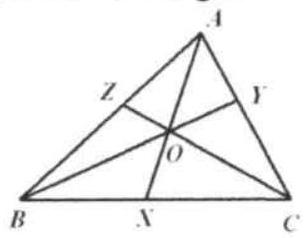
\includegraphics[width=\textwidth]{images/129.jpg}

\section*{Solution}
Solution not available.

\end{document}
